\chapter{Introducción}\label{cap:introduccion}

\section{Robótica y tecnologías afines}\label{sec:contextoIntroduccion}
Durante mucho tiempo la robótica ha sido una disciplina muy alejada y poco accesible al público, tanto por su coste económico, como por el difícil acceso a recursos académicos (manuales teóricos o recursos humanos). Esto la ha convertido, en lo que se refiere a una visión popular, en una disciplina de lujo accesible a unos pocos privilegiados económica o académicamente (agencias espaciales, grandes corporaciones, robots súper funcionalea, etc) llegando incluso a ser más cercana a la ciencia ficción que a la ingeniería corriente. No era vista como una disciplina científica cercana a la que poder dedicarse, mucho menos como una asignatura accesible a estudiantes jóvenes o universitarios. \\
Además, el  ``resultado'' de la robótica tampoco era visto como algo real, sino como ciencia ficción o productos de lujo económico. No se concebían los robots como algo adaptable a la vida corriente ni se pensaba en soluciones \textit{robóticas} a problemas reales. A esta visión de la robótica y de los robots ha contribuido en gran medida la literatura y el cine, creando en el imaginario popular robots humanoides indistinguibles de personas reales, completamente independientes y funcionales o inteligencias artificiales utilizadas para viajes espaciales que crecen y se desarrollan al margen de la humanidad.\\

Durante los últimos años, no obstante, se ha observado un cambio de paradigma, impulsado desde el mundo de la ingeniería y el pragmatismo comercial. Los robots han dejado de verse como ``humanos electrónicos'', convirtiéndose poco a poco en una definición más realista, como un proceso electrónico programado para cumplir una o varias funciones interactuando con el medio. Tenemos varios ejemplos de esta nueva definición de robótica:

\begin{description}
	\item [Automatismos.] También llamados \textit{\textbf{bots}}, son un robot sin una capa física que funciona de forma independiente recogiendo datos, procesándolos y respondiendo a ellos de forma \textit{inteligente}. Algunos ejemplos son los aplicativos de \textit{metadata} (muy extendidos) o los conocidos ``chat de ayuda'' en las aplicaciones web (asistentes de ayuda al cliente). Otro ejemplo de uso de estos automatismos son los procesos de seguridad de los vehículos modernos, que se mantienen recogiendo datos del medio  para ofrecer una capa añadida de seguridad frente a posibles errores humanos (velocidad, proximidad y velocidad de otros vehículos, distancias entre carriles, etc).\\
	Una de las características principales de estos \textit{procesos robotizados} es que arrancan sin requerir interacción. Aparte de que una vez funcionando respondan a peticiones o estímulos humanos, no requieren de que se les ``ordene'' encenderse. Siempre pueden apagarse, por motivos obvios de seguridad, pero volverán a arrancar con la misma configuración y, lo más importante, sin necesitar de ningún \textit{reset} o configuración inicial.
	
	\begin{figure}[h]
		\centering
		\begin{subfigure}
			[Seguridad robotizada en un coche]{
			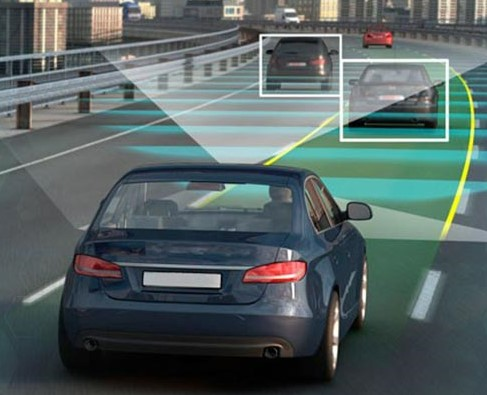
\includegraphics[scale=0.5]{coche.jpg}
			\label{img:coche}
		}
		\end{subfigure}
	\begin{subfigure}
		[Chatbot de ayuda comercial]{
			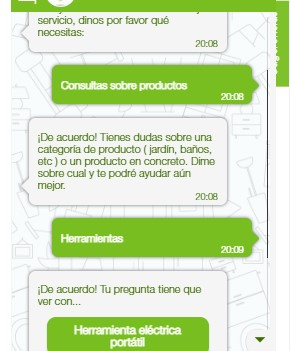
\includegraphics[width=6cm]{chatbot.jpg}
			\label{img:chatbot}
		}
	\end{subfigure}
	\caption{Ejemplos de automatismos}
	\label{img:bots}
	\end{figure}

	\item [Internet Of Things.]\footnote{Internet de las cosas} Muy escuchado, aunque popularmente no se conecte con la robótica. La idea básica del IOT es añadirle conexión a Internet a objetos de uso diario, con los objetivos de:
	\begin{itemize}
		\item Añadir funcionalidades que requieren de conexión online. Por ejemplo, un reloj inteligente con el que poder atender mensajes o llamadas o pagar compras. El usuario interactúa con estas funcionalidades para obtener una respuesta, aunque la aplicación se mantiene funcionando siempre. Es decir, funciona esperando un estímulo al cual responder.
		\item Recoger datos para procesarlos y ofrecer información añadida en función de esos datos. El mismo reloj inteligente recoge datos de sueño, y te muestra la calidad y horas de éste. Con estas funciones no es necesario interactuar sino que están preparadas para recoger datos siempre que estén disponibles y mostrar al usuario los resultados de los procesos que tenga programados.
	\end{itemize}
	El IOT funciona con procesos robotizados, programados para recoger datos de forma automática o responder a estímulos del medio, que siguen las mismas normas antes mencionadas: se mantienen funcionando (siempre que no se les apague expresamente) sin necesidad de configuraciones añadidas; su programación se encarga de ello. Ciertamente, muchos objetos con IOT necesitan de datos iniciales para su puesta en marcha debido a que los datos recogidos son biométricos y necesitan de un contexto inicial para el procesamiento de datos. Podemos ver varios ejemplos de IOT en la figura \ref{img:IOT}.
	\begin{figure}[h]
		\centering
		\begin{subfigure}
			[Información de la calidad del sueño proporcionada por un reloj inteligente] {
			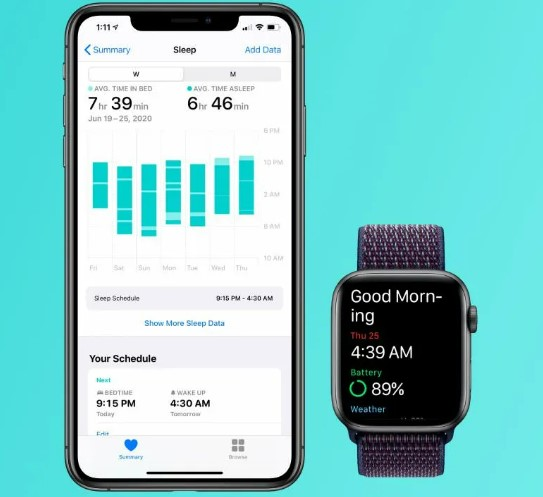
\includegraphics[scale=0.5]{IOT1.jpg}
			\label{img:IOT1}}
		\end{subfigure}
		\begin{subfigure}
			[Báscula inteligente que procesa los datos almacenados] {
			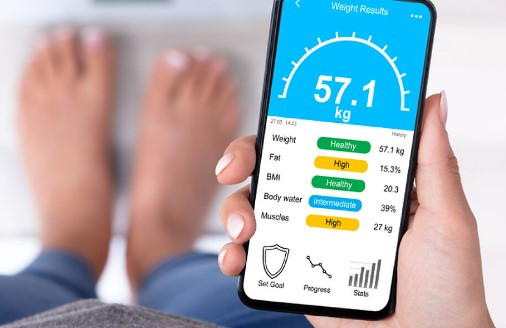
\includegraphics[scale=0.5]{IOT2.jpg}
			\label{img:IOT2}}
		\end{subfigure}
		\newline
		\begin{subfigure}[c]
			[Aplicación conectada a un sensor de glucosa para controlar el nivel de azúcar] {
			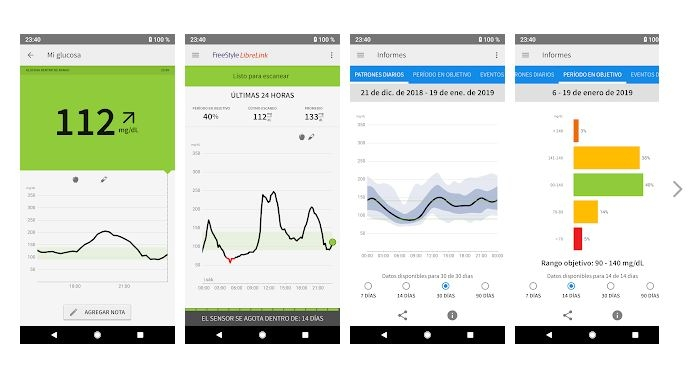
\includegraphics[scale=0.5]{IOT3.jpeg}
			\label{img:IOT3}}
		\end{subfigure}
		\caption{Ejemplos de IOT}
		\label{img:IOT}
	\end{figure}

	\item [Domótica.] Posiblemente la utilidad robótica más extendida a día de hoy. Cada vez más unida al IOT, aunque no lo requiere expresamente. Viene del significado latino de 'casa' y engloba a todo sistema o automatismo diseñado para cumplir una función que facilite una tarea doméstica o le añada funcionalidad. Tenemos sistemas de seguridad, aspiradores, electrodomésticos que se comportan diferente dependiendo de las circunstancias (cantidad de agua de una lavadora, o temperatura de un frigorífico), control de luces con aplicaciones móviles (tanto con Internet como sin él), controles de accesos, etc. Todo esto son procesos robotizados (robots al fin y al cabo) que utilizan información del medio para reaccionar de una u otra manera. Esta información puede provenir de sensores (la lavadora o el frigorífico) o recibirla del usuario/a (apagar o encender las luces, la TV o la alarma). En la figura \ref{img:domotica} tenemos ejemplos de aplicaciones domóticas.
	\begin{figure}[h]
		\centering
		\begin{subfigure}
			[Robot aspirador] {
				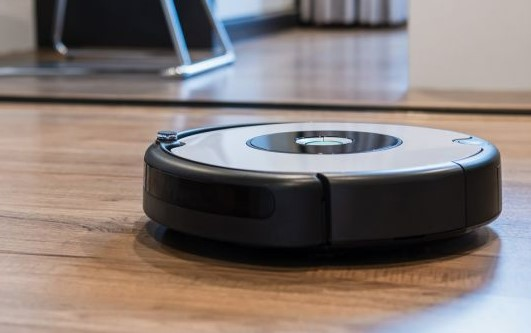
\includegraphics[scale=0.5]{domotica1.jpg}
				\label{img:domo1}}
		\end{subfigure}
		\begin{subfigure}
			[Elementos para control inteligente de luces] {
				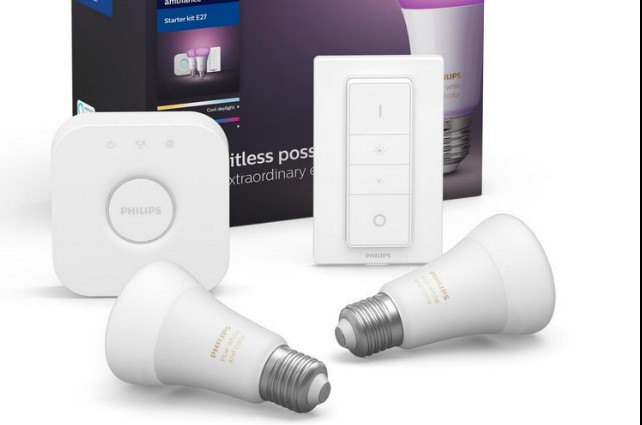
\includegraphics[scale=0.5]{domotica2.jpg}
				\label{img:domo2}}
		\end{subfigure}
		\caption{Ejemplos de domotica}
		\label{img:domotica}
	\end{figure}
	\item [Inteligencia Artificial.] Uno de los grandes trabajos respecto al cambio de visión de la robótica ha sido conseguir cambiar el ideario de Inteligencia Artificial y de separarlo del concepto de robot. Lejos del concepto que tradicionalmente se tenía de Inteligencia Artificial (como hemos comentado, en parte culpa de la ciencia ficción, por ejemplo el robot M.A.D.R.E. de la pelicula \textit{Alien}), podemos encontrar inteligencias artificiales habitualmente en nuestro día a día. Por ejemplo, los asistentes virtuales de diferentes fabricantes (Google, Amazon o Apple) aprenden del medio en mayor o menor medida y son capaces de buscar una respuesta que no tienen pre-programada (un ejemplo de estas IA está en la figura \ref{img:alexa}), o los programas de procesamiento de \textit{big data} que se realimentan con los datos que recogen y de sus propios resultados para afinar esos mismos algoritmos de procesamiento.
	\begin{figure}[h]
		\centering
		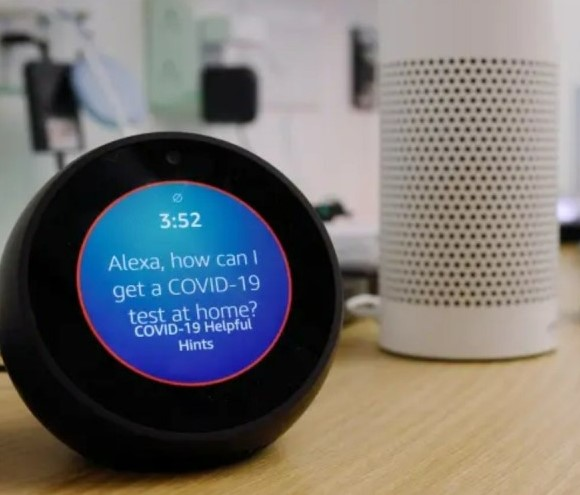
\includegraphics[scale=0.5]{alexa.jpg}
		\caption{Inteligencia Artificial}
		\label{img:alexa}
	\end{figure}
	
	\item [Juguetes robots] Finalmente, llegamos a la aplicación más reconocible como ``robot'' propiamente dicho, también muy lucrativa. La robótica ha tenido un gran impulso en el ocio, creándose diferentes juguetes tanto para niños como para adultos. Se han convertido de ser un juguete de élite a tener variedad de opciones, con diversas funcionalidades, y accesibles a más variedad de costes. Esta accesibilidad de la robótica en el ocio ha contribuido en gran medida a esa transformación de la robótica y a incluirla en nuestras vidas, dando lugar a muchas otras aplicaciones. Una aplicación robótica que empieza siendo un juguete, puede convertirse en algo mucho más práctico e importante. Por ejemplo, los drones (en la figura \ref{img:drones}), que tienen cada vez más utilidades diferentes.
	
	\begin{figure}[h]
		\centering
		\begin{subfigure}
			[Drone teledirigido orientado al ocio grabando deporte] {
				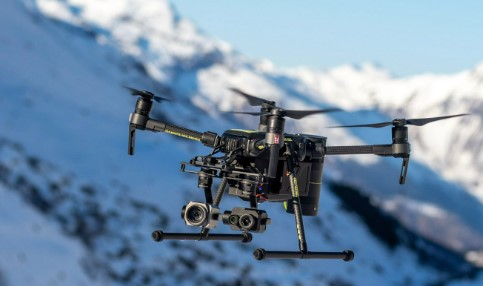
\includegraphics[width=0.33\textwidth]{droneski.jpg}
				\label{img:drone1}}
		\end{subfigure}
		\begin{subfigure}
			[Drone de ayuda humanitaria] {
				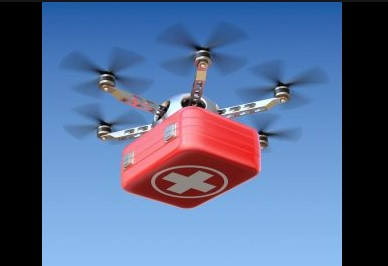
\includegraphics[width=0.33\textwidth]{dronerescate.jpg}
				\label{img:drone2}}
		\end{subfigure}
		\caption{Diferentes ejemplos de uso para un mismo tipo de robot}
		\label{img:drones}
	\end{figure}
	
	
	En cuanto a este Trabajo Fin de Grado, esta aplicación es la que más nos interesa.
\end{description}

\section{Robótica Educativa}


Estos cambios por parte de la industria y avances por parte de la ingeniería han contribuido a acercar la robótica a las personas de a pie, sobre todo a las generaciones más jóvenes, facilitando el acceso a recursos con los que aprender y creando un interés por ello. Es muy notable el abaratamiento de los diversos componentes, así como de los productos finales, y la introducción de esta disciplina en los diferentes niveles educativos (sobre todo en estudios universitarios). El hecho que más gente tenga acceso a los recursos necesarios, y tenga desde joven los conceptos inculcados, contribuye a aumentar las aplicaciones prácticas en todos los ámbitos, y a resolver problemas en los que anteriormente, al no ser una disciplina extendida, quizá nadie había reparado. \\

Sin embargo, y a pesar de todo este trabajo realizado y todo lo conseguido, aún queda mucho por trabajar. El principal problema para que una persona se ponga a aprender cómo programar un \textit{comportamiento robótico} es que debe aprenderlo desde cero, sin haber tenido un aprendizaje progresivo como con el resto de enseñanzas. La Matemática, la Física o la Química, se enseña con niveles progresivos de dificultad, desde edades muy tempranas con las metodologías y conceptos ampliamente discutidos y formulados, para poder llegar a aplicaciones más avanzadas. Nadie espera que una persona sin conocimiento ninguno de estas materias, arranque  un curso de, por ejemplo, Cálculo Diferencial, Matemática Discreta o Teoría Gravitatoria. Es decir, se \textit{educa} al cerebro desde el principio, cuando más capacidad de aprendizaje se tiene, para adaptarse a nuevos conceptos y poder aprenderlos gradualmente. \\
\par Con la robótica y el pensamiento computacional no se ha seguido ese orden lógico. La mayoría de los estudiantes que aprenden Programación, Computación o Algoritmia lo hacen a edades más avanzadas, ya sea por su cuenta o con educación reglada. Si esta educación comenzara, como otras disciplinas, con los alumnos y alumnas siendo mucho más jóvenes y avanzara con ellos durante las siguientes etapas educativas, se conseguiría que llegaran a las más avanzadas mucho más preparados. Además despertaría en muchos más estudiantes la curiosidad por estas carreras, tanto profesional como educativamente.\\

Para responder a esta necesidad han surgido varios entornos de robótica educativa orientada a niños y niñas. Los principios fundamentales de todos ellos son parecidos. Buscan la simplicidad, evitando complicados lenguajes de programación, y crear una plataforma visual y llamativa con la que llamar la atención de los niños. Algunos de ellos son:
\begin{description}
	\item [OpenRoberta]\cite{Roberta} Cuenta con la ventaja de ser una herramienta completamente \textit{online}, con capacidad de almacenamiento en la nube para guardar los avances. La programación de los robot se realiza en un lenguaje visual, sin sintaxis. La característica principal de esta herramienta es la posibilidad de programar algunos robots de forma \textit{simulada}, además del robot real. Así es posible probar un ejercicio mucho más rápidamente que con el robot real, o incluso programar comportamientos sin tener un robot disponible. Además, tiene disponibles varios robots de diferentes fabricantes basados en diferentes placas base (Arduino o Java, por ejemplo). 	
	\begin{figure}[h]
		\centering
		\includegraphics[scale=0.4]{RobertaSimulado.jpg}
		\caption{Entorno simulado de OpenRoberta}
		\label{img:roberta}
	\end{figure}
	
	\item [Lego Boost]\cite{Lego} La famosa empresa de juegos de bloques de construcción tiene varios sets para la construcción de robots orientados a diferentes edades. El robot se programa con una aplicación para dispositivos móviles, y no usa un lenguaje sino bloques pictográficos con los que programar los diferentes bloques, lo que lo hace disponible para niños y niñas muy pequeños. Otra ventaja es que es compatible con el resto de bloques de construcción de la marca, por lo que se puede construir un robot personalizado.
	\begin{figure}[h]
		\centering
		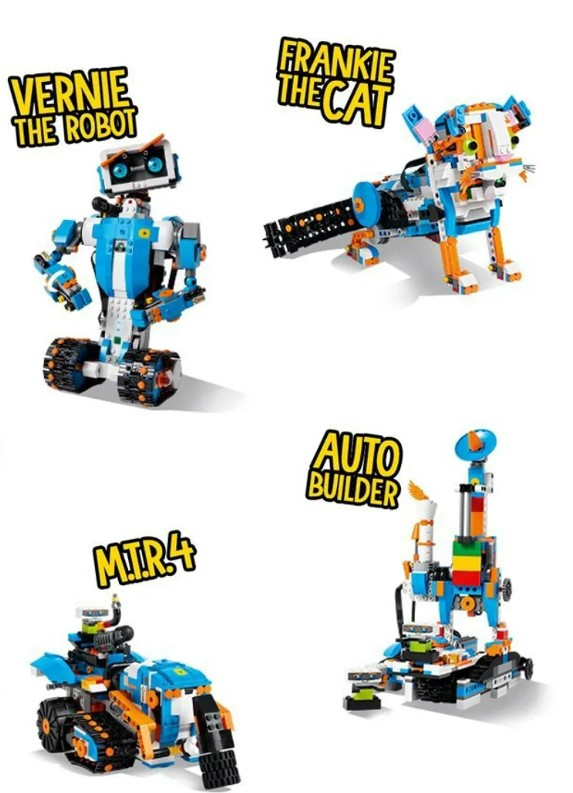
\includegraphics[scale=0.4]{lego.jpg}
		\caption{Robots con el kit de Lego}
		\label{img:lego}
	\end{figure}
	
	\item [Kibotics]\cite{kibotics} Desarrollada por JdeRobot, está orientada a la robótica educativa a todos los niveles. Ofrece una plataforma donde programar robots, tanto reales como simulados, en Python y Scratch, y cursos en ambos lenguajes para alumnos de diferentes edades. Al disponer de un entorno de programación simulada, no es necesario tener un robot físico para los cursos. 
	\begin{figure}[h]
		\centering
		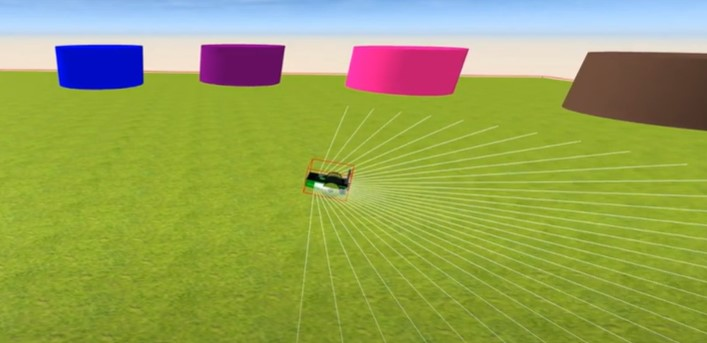
\includegraphics[scale=0.6]{kibotics.jpg}
		\caption{Ejercicio de robótica simulada de un curso de Kibotics}
		\label{img:kibotics}
	\end{figure}
	\item [mBlock]\cite{mblock} Desarrollado por Makeblock \cite{makeblock}, es una de las plataformas para programación de robots educativos más extendida. Es una plataforma, con versiones tanto \textit{online} como instalables para dispositivos móviles y PC, que utiliza el lenguaje de programación para niños Scratch. Contiene los módulos de programación para robots de Makeblock y placas Arduino (puede verse en la figura \ref{img:mblockplacas}).
	
	\begin{figure}[h]
		\centering
		\begin{subfigure}
			[Versión online de mBlock] {
				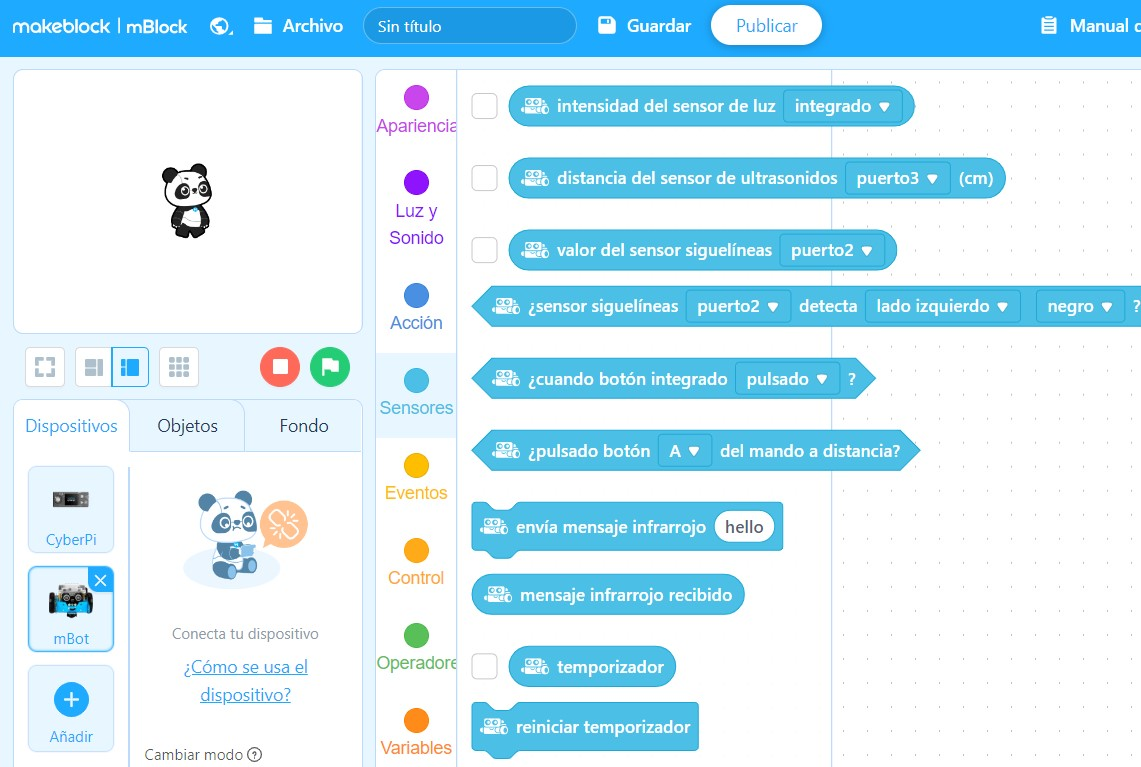
\includegraphics[width=0.6\textwidth]{mblockweb.jpg}
				\label{img:mblockonline}
			}
		\end{subfigure}
		\begin{subfigure}
			[Placas base y robots disponibles en mBlock] {
				\includegraphics[scale=0.7]{mblockPlacas.png}
				\label{img:mblockplacas}
			}
		\end{subfigure}
		\caption{mBlock}		
	\end{figure}

	
\end{description}
\vspace{2cm}
\par Con la idea de introducir en la robótica a niños y jóvenes como principal foco de atención, el propósito de este Trabajo Fin de Grado es ofrecer una propuesta para la enseñanza de robótica y programación a alumnos y alumnas sin conocimientos previos, tanto de Educación Primaria como Secundaria. Para ello se ha utilizado un robot educativo llamado mBot, del fabricante Makeblock \cite{makeblock}, que cumple los requisitos de simplicidad y accesibilidad que requiere el trabajar con niños y niñas. Está especialmente preparado para la enseñanza sin dejar de ser un \textit{juguete}, ya que buscamos despertar el interés y convencer de la facilidad de una disciplina a menudo vista como especialmente complicada y aburrida.

Este proyecto estará compuesto de dos partes. La primera será la creación de una manera sencilla de programar el mBot en el lenguaje de programación Python, siendo éste mucho más sencillo que el lenguaje nativo de la placa base del robot. Se explicará el proceso seguido para desarrollar esta solución, poniendo énfasis en detallar los pasos necesarios para replicarlo, utilizarlo en clases reales con alumnos e incluso ampliarlo. En la segunda parte encontraremos una propuesta completa de uso práctico de esta plataforma, con ejercicios detallados y soluciones de referencia, aumentando el nivel de dificultad progresivamente y con objetivos conceptuales claramente marcados.

Obtendremos así una forma para enseñar de forma accesible y fácil conceptos complejos como algoritmia, programación o metodologías de desarrollo de Software sin necesidad de explicaciones teóricas y poco adaptadas a edades alrededor de los 7-15 años.


\section{Antecedentes}\label{sec:antecedentes}

Dentro de la Universidad Rey Juan Carlos, la organización de software abierto para robótica JdeRobot y particularmente el proyecto PyBoKids \cite{JdeRobot} han servido de antecedente ideológico a este Trabajo Fin de Grado. Ofrecen recursos para robótica educativa, teniendo en cuenta diferentes robot, diferentes plataformas y orientado a varios rangos de edades pre-universitarias.\\

En este Trabajo Fin de Grado hemos tomado del proyecto PyBoKids el propósito educativo, y el concepto de \textit{middleware entre el estudiante y el robot}. Hemos contado como base con la experiencia de un curso escolar de clases extracurriculares de robótica con alumnos de Educación Primaria realizado en el Colegio Nuestra Señora de Rihondo, en Alcorcón. Se comprobó la efectividad del lenguaje Scratch para la enseñanza de robótica y el desarrollo del pensamiento computacional. También se comprobaron las necesidades y limitaciones existentes en caso de querer continuar el curso con un lenguaje textual. De ahí salió la necesidad de una solución educativa sencilla, lo más accesible posible en cuanto a herramientas y conceptos, y con objetivos marcados y preparados para que cualquiera pueda utilizarlos.


